% arara: pdflatexmkhalt: {shell: yes}
% arara: makechapters: {compileAll: no, items: [chapters/cosmic-rays, chapters/station, chapters/cluster, chapters/processing]}

% chapters/cosmic-rays,
% chapters/station,
% chapters/cluster,
% chapters/processing,

% chapters/analysis,
% chapters/conclusions,
% chapters/coordinates,
% chapters/network,
% chapters/outreach,
% chapters/pmt_design,
% chapters/simulations,
% chapters/software,
% chapters/summary

\documentclass[a4paper, 11pt, oneside]{book}
\usepackage{a4wide}

\usepackage[T1]{fontenc}	% e.g. For bold small caps
\usepackage[utf8]{inputenc}     % For `Łódź

\usepackage[dutch, english]{babel}
\usepackage{fouriernc}  % Use NC Schoolbook font for math
%\usepackage{tgschola}
\usepackage[svgnames]{xcolor}
% Libertine (serif), Biolinum (sans-serif), and LibertineMono (mono) fonts
\usepackage[libertine]{quotchap}
\usepackage[font={small, sf}, labelfont={bf}, labelsep=endash]{caption}
%\newcommand{\captitle}[1]{\textsmaller{\MakeUppercase{#1}}}
\newcommand{\captitle}{}
\DeclareCaptionFormat{thesis}{\sansmath #1#2#3}
\captionsetup{format=thesis}
\usepackage{fancyhdr}
\pagestyle{fancy}
\fancyhead{}
\fancyfoot{}
\fancyhead[LE, RO]{\thepage}
\fancyhead[RE]{\nouppercase\leftmark}
\fancyhead[LO]{\nouppercase\rightmark}

% Prevent widow and orphan lines
\widowpenalty = 10000
\clubpenalty = 10000

\setcounter{tocdepth}{2}
\setlength{\headheight}{14.5pt}
\renewcommand{\topfraction}{.85}
\renewcommand{\textfraction}{.15}
\renewcommand{\floatpagefraction}{.7}

\renewcommand{\chapterheadstartvskip}{\vspace*{-1cm}}

% Fix for layout problems
\makeatletter
\renewcommand{\@pnumwidth}{2em}
\renewcommand{\@tocrmarg}{4em}
\makeatother

\usepackage{xspace}
\usepackage{relsize}
\usepackage{setspace}

% TikZ
%\usepackage{graphicx}  % Already imported by TikZ
\usepackage{tikz}
\pgfkeys{/artist/width/.initial=.67\linewidth}
\usetikzlibrary{calc, arrows, chains, scopes, fit, decorations.pathmorphing,
                decorations.markings, intersections, pgfplots.groupplots,
                external, shapes, spy}
\usepackage{pgfplots}
\usepackage{tikz-3dplot}
\pgfplotsset{compat=1.3}
\usepgfplotslibrary{polar}
\tikzexternalize
\tikzsetexternalprefix{tikz/}

\usepackage[detect-all, binary-units, separate-uncertainty,
            retain-unity-mantissa=false]{siunitx}
\usepackage{amsmath}
\usepackage{epigraph}  % For typesetting quotations
\usepackage{hepnames}  % For typesetting particles
\usepackage[backend=biber, style=nature]{biblatex}
\addbibresource{articles/general/references.bib}
\addbibresource{articles/1_cosmic-rays/1_cosmic-rays.bib}
\addbibresource{articles/2_station/2_station.bib}
\addbibresource{articles/3_cluster/3_cluster.bib}
\addbibresource{articles/4_processing/4_processing.bib}
% \addbibresource{articles/5_dataset/5_dataset.bib}
\addbibresource{articles/6_reconstructions/6_reconstructions.bib}
% \addbibresource{articles/7_501_510/7_501_510.bib}
% \addbibresource{articles/8_sciencepark/8_sciencepark.bib}
% \addbibresource{articles/9_conclusions/9_conclusions.bib}
% \addbibresource{articles/a1_software/a1_software.bib}
% \addbibresource{articles/a2_coordinates/a2_coordinates.bib}

%\usepackage{comment}
%\includecomment{comment}
\usepackage{sidecap}
\usepackage{booktabs}
\usepackage{minted}    % For nice source code rendering
\usepackage{sansmath}
\sisetup{text-sf=\sansmath}
\usepackage{eurosym}
\usepackage{pdfpages}  % Include pages from other pdfs

% Keep this one the last packages, to let it overrule previous declarations
\usepackage[pdfusetitle]{hyperref}


\usepackage{shape-datastore}

% Projects
\newcommand{\hisparc}{\textsmaller{HiSPARC}\xspace}
\newcommand{\kascade}{\textsmaller{KASCADE}\xspace}
\newcommand{\nikhef}{\textsmaller{Nikhef}\xspace}
\newcommand{\kmnet}{\textsmaller{KM3NeT}\xspace}
\newcommand{\knmi}{\textsmaller{KNMI}\xspace}
\newcommand{\lhc}{\textsmaller{LHC}\xspace}
\newcommand{\ta}{\textsmaller{TA}\xspace}

% Software
\newcommand{\sapphire}{\textsmaller{SAPPHiRE}\xspace}
\newcommand{\pysparc}{\textsmaller{PySPARC}\xspace}
\newcommand{\jsparc}{\textsmaller{jSparc}\xspace}
\newcommand{\api}{\textsmaller{API}\xspace}
\newcommand{\daq}{\textsmaller{DAQ}\xspace}
\newcommand{\git}{\textsmaller{git}\xspace}
\newcommand{\aires}{\textsmaller{AIRES}\xspace}
\newcommand{\corsika}{\textsmaller{CORSIKA}\xspace}
\newcommand{\dspmon}{\textsmaller{DSPMon}\xspace}
\newcommand{\esd}{\textsmaller{ESD}\xspace}

% Physics
\newcommand{\gzk}{\textsmaller{GZK}\xspace}
\newcommand{\gz}{\textsmaller{GZ}\xspace}
\newcommand{\ism}{\textsmaller{ISM}\xspace}
\newcommand{\igm}{\textsmaller{IGM}\xspace}

% Web services
\newcommand{\github}{\textsmaller{GitHub}\xspace}
\newcommand{\travis}{\textsmaller{Travis CI}\xspace}
\newcommand{\coveralls}{\textsmaller{Coveralls}\xspace}
\newcommand{\codecov}{\textsmaller{Codecov}\xspace}
\newcommand{\pypi}{\textsmaller{PyPI}\xspace}

% Data formats
\newcommand{\hdf}{\textsmaller{HDF5}\xspace}
\newcommand{\csv}{\textsmaller{CSV}\xspace}
\newcommand{\tsv}{\textsmaller{TSV}\xspace}
\newcommand{\json}{\textsmaller{JSON}\xspace}

% Languages
\newcommand{\javascript}{\textsmaller{JavaScript}\xspace}
\newcommand{\python}{\textsmaller{Python}\xspace}
\newcommand{\fortran}{\textsmaller{FORTRAN}\xspace}
\newcommand{\labview}{\textsmaller{LabVIEW}\xspace}

% ...
\newcommand{\mip}{\textsmaller{MIP}\xspace}
\newcommand{\mpv}{\textsmaller{MPV}\xspace}
\newcommand{\ldf}{\textsmaller{LDF}\xspace}
\newcommand{\utc}{\textsmaller{UTC}\xspace}

% Hardware
\newcommand{\hisparcii}{\textsmaller{HiSPARC II}\xspace}
\newcommand{\hisparciii}{\textsmaller{HiSPARC III}\xspace}
\newcommand{\adc}{\textsmaller{ADC}\xspace}
\newcommand{\adcs}{\textsmaller{ADC}s\xspace}
\newcommand{\fpga}{\textsmaller{FPGA}\xspace}
\newcommand{\pmt}{\textsmaller{PMT}\xspace}
\newcommand{\pmts}{\textsmaller{PMT}s\xspace}
\newcommand{\gps}{\textsmaller{GPS}\xspace}
\newcommand{\pps}{\textsmaller{PPS}\xspace}
\newcommand{\osm}{\textsmaller{OSM}\xspace}
\newcommand{\ctp}{\textsmaller{CTP}\xspace}
\newcommand{\ctd}{\textsmaller{CTD}\xspace}
\newcommand{\senstech}{Sens-Tech\xspace}

% References
\usepackage[capitalise, noabbrev]{cleveref}

% Redefine to ensure proper spacing (fouriernc)
\DeclareSIUnit{\electronvolt}{\ensuremath{\mathrm{e\!\!\:V}}}

\DeclareSIUnit{\unitsigma}{\ensuremath{\sigma}}
\DeclareSIUnit{\mip}{\textsmaller{MIP}}
\DeclareSIUnit{\adc}{\textsmaller{ADC}}

\DeclareSIUnit{\gauss}{G}
\DeclareSIUnit{\parsec}{pc}
\DeclareSIUnit{\year}{yr}

% Equations
\newcommand{\ud}{\mathrm{d}}
\newcommand{\diff}{\mathop{}\!\ud}

\renewcommand{\EUR}[1]{\euro\,\num{#1}}

% Disable slow parts for faster draft output
% \newcommand{\longprocess}[1]{}
\newcommand{\longprocess}[1]{#1}


% Disable this for draft output (it is really slow)
%\usepackage[babel]{microtype}

% Only activate this for draft output
%\renewcommand{\longprocess}[1]{}

\onehalfspacing

\title{HiSPARC}
\author{A.~P.~L.~S.~de Laat}


\begin{document}

%\makeatletter
%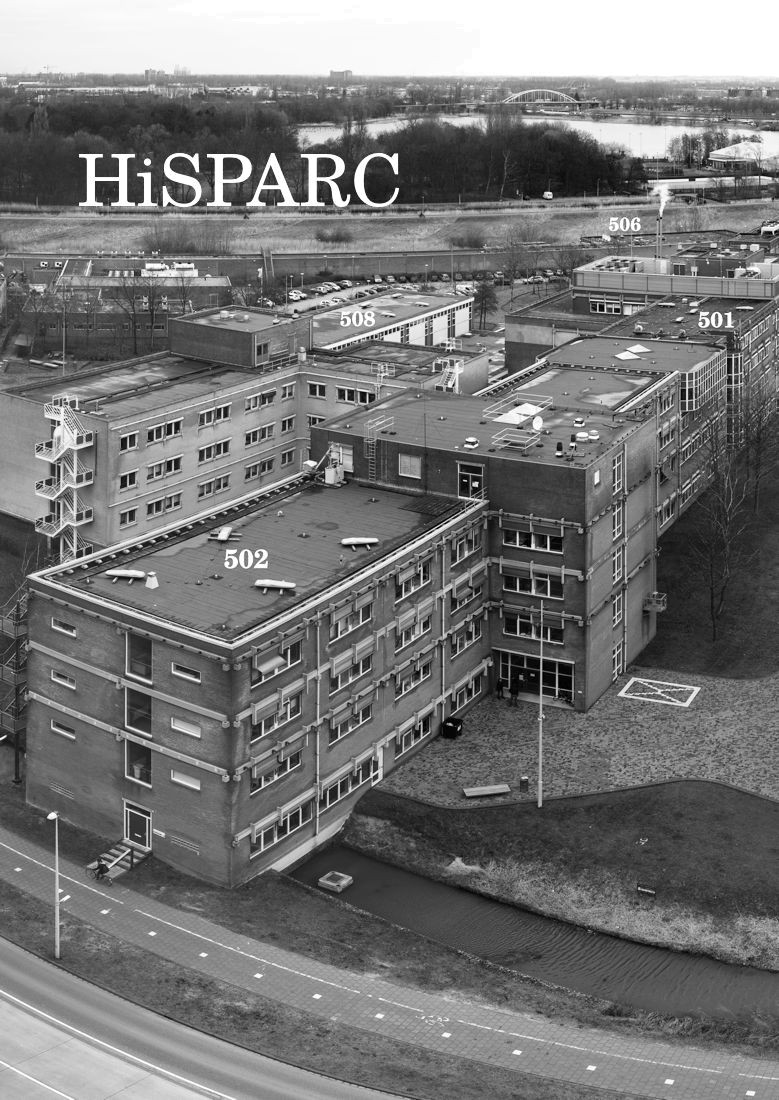
\includepdf{cover/crop-cover}
%\makeatother

%\thispagestyle{empty}
%\cleardoublepage

%\frontmatter

%\thispagestyle{empty}

\begin{center}

\vspace*{2cm}

\textlarger[3]{\hisparc}
\\[1em]
\textlarger[1]{RECONSTRUCTIONS}
\end{center}

\clearpage

\vspace*{\fill}

\noindent
Dutch title: \emph{\hisparc: reconstructies.}

\vspace{1cm}

\noindent
ISBN: 153957 \\
DOI: 153957

\vspace{3cm}


\includegraphics[height=2.5cm]{figures/logo_FOM_zw}
\hfill

\includegraphics[height=2cm]{figures/logo_NWO_zw}

\vspace{.5cm}

\noindent
This work is part of the research programme of the Foundation for
Fundamental Research on Matter (FOM), which is part of the Netherlands
Organisation for Scientific Research (NWO).  It was carried out at the
National Institute for Subatomic Physics (Nikhef).


% Actual 'titlepage'

\cleardoublepage
\thispagestyle{empty}

\begin{center}

\vspace*{2cm}

\textlarger[3]{\hisparc}
\\[1em]
\textlarger[1]{RECONSTRUCTIONS}


\begin{onehalfspace}

\vspace{2cm}

PROEFSCHRIFT

\vspace{2cm}

.....\\

\vspace{1cm}

door

\vspace{1cm}

Adriaan Paul Ludovic Siem de Laat\\
geboren op 16 september 1987\\
te Amsterdam

\end{onehalfspace}
\end{center}


\newpage


\noindent
Dit proefschrift is nog niet goedgekeurd.
\begin{tabbing}
Promotor: \\
Assistent-promotor:
\end{tabbing}


%\cleardoublepage

%\vspace*{1in}
%\hfill
%\parbox{5cm}{
%\textlarger{\textit{Voor }}\\
%\textsmaller{...}
%\\[10pt]
%\textlarger{\textit{Voor }}\\
%\textsmaller{...}
%\\[10pt]
%\textlarger{\textit{Voor }}\\
%\textsmaller{...}
%}

\tableofcontents

\mainmatter
\renewcommand{\epigraphflush}{flushleft}
\chapter{\hisparc Experiment}
\label{ch:hisparc-experiment}

Detecting cosmic-ray extensive air showers with affordable detectors
using plastic scintillators and photomultiplier tubes, the design is
explained in \secref{sec:detector_design}.

Large network area, sparse array. Detector station locations are often
limited to high-school roofs or universities and other institutions.
Some stations, however, are located at the homes of participants, e.g.
a garage roof [photo nijmegen/ucu?].


\section{Network status}

Currently there are 120 active \hisparc stations in the world. Stations
are located at high schools and research institutes in the Netherlands,
United Kingdom and Denmark.

[plot for number of active stations from 2004-ish untill now]

\begin{figure}
    \centering
    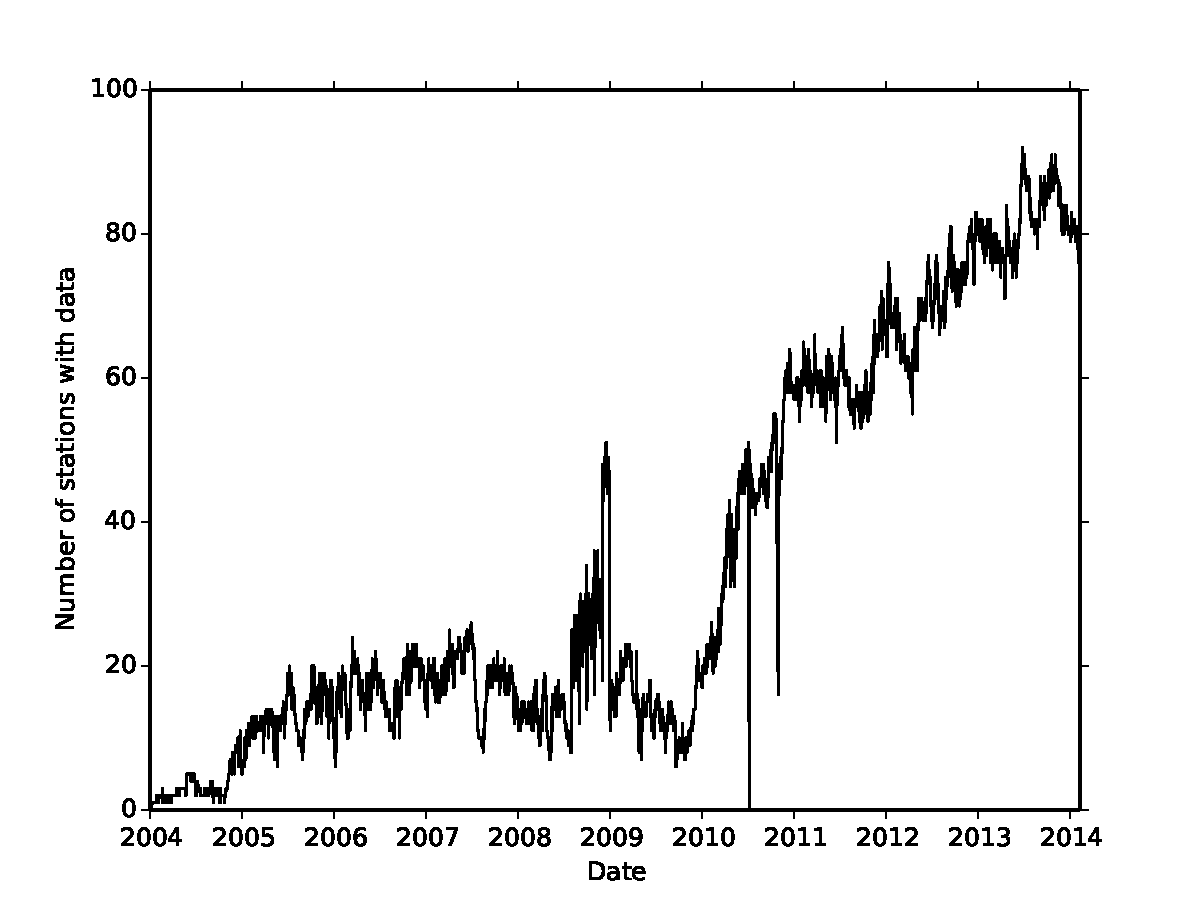
\includegraphics[width=0.7\linewidth]
        {plots/network/number_of_stations_with_data_per_day}
    \caption{\captitle{Active stations over time.} The number of active
             stations per day from January 1st 2004 until now.}
    \label{fig:number_of_stations_with_data_per_day}
\end{figure}


\subsection{International}

In Germany one of our stations (70001) was placed inside the \kascade
experiment in Karlsruhe on July 1, 2008. This was done to calibrate and
test the direction reconstruction accuracy of a single \hisparc station.
Although the \kascade-GRANDE experiment officially shut down on March
30, 2009, it was kept active until November, 26th 2011 as a test
facility for some test setups, including our detector. The \kascade
experiment triggered the \hisparc station when it detected a shower. It
was triggered more than \num{9e7} (in publicdb, more on external hdd?
and in `/databases/kascade`?) times in this period. The detectors have
been repurposed and are now part of station 508 on the Science Park.

Since 2007 there has been a \hisparc station in
Denmark. There are currently 3 operational stations at the Aarhus
University. These stations are managed by Uffe Amelung Fredens.
Fredens is writing student materials for Danish high school students.

In Bristol, England a new cluster started to form around Bristol in
March 2012. This was initiated by Dr. Jaap Velthuis who is the cluster
coordinator for Bristol. Since then schools in Bristol, Bath, Swindon
and Chippenham have joined the network. More on the way..

[Finland/Spain.. perhaps?]


\section{Detector design}
\label{sec:detector_design}

\subsection{Scintillator}

\SI{100 x 50 x 2}{\centi\meter} cuboid of plastic scintillator, with the
base polyvinyltoluene and the fluor anthracene. 


\subsection{Photo multiplier}

Performance
Nikhef designed high-voltage voltage-divier circuit.
Cockcroft-Walton voltage multiplier circuit.
High linearity?


\subsection{HiSPARC electronics}

Readout electronics. Two channels, each with two ADCs which readout a
signal up to \SI{-2}{\volt}. And return a 12-bit value (4096 ADCcounts
range). Each ADC is sampled at 200 Mhz, using two ADCs per channel gives
400 Mhz (2.5 ns) per channel. Nikhef designed. Some (derivatives) used
in other experiments.

Multiple versions, Latest version \hisparciii. New software needed,
remote firmware updates.


\section{Station}

Multiple detectors connected to \hisparc electronics makes a station.

\begin{figure}
    \centering
    \input{plots/hisparc-experiment/4_detector_station}
    \caption{\captitle{Standard 4-detector station layout.} The colored
             rectangles represent the scintillator detectors.}
    \label{fig:4_detector_station}
\end{figure}

\chapter{Cosmic-rays}
\label{ch:cosmic-rays}

\chapter{Software}
\label{ch:software}

\section{\github}

Our code has transitioned from bazaar to \git, a different distributed
version control system. This made it possible to use the service \github
to host our projects. \github provides a web-interface to manage
projects, keep track of issues and pull requests.

When we were using bazaar our repositories were hosted on a Nikhef
server, this made it difficult for others to participate and contribute.
On \github the software has been open sourced and can be downloaded with
a single click, on any system.

\github also provides webpage hosting of static pages for repositories,
called \github Pages. We use it to host software documentation and
compiled version of the teaching materials, for which the sources are
also on \github.


\section{Structure}

Since the code can now be easily accessed by anyone we cleaned up the
code to be more consistent and conform to a coding style. For \python we
try to conform to Python Enhancement Proposal (PEP) 8 - Style Guide for
Python Code.


\section{Repositories}

This is a list of the different repositories.

\begin{verbatim}
Data analysis/presentation
sapphire - SAPPHiRE, a framework for HiSPARC
pysparc - HiSPARC DAQ implemented in Python
publicdb - The HiSPARC Public Database
jsparc - Javascript library and coincidences analysis
gz-sim - Gerasimova-Zatsepin effect simulation
framework - (deprecated) HiSPARC tools
correlation - Data correlation analysis
interaction-position - Calculate possible interaction positions from detection timestamps
practica - project by Niek?
data-quality - Data quality checks
topaz PRIVATE - Scripts for small analyses with HiSPARC data
tijdtest PRIVATE - Analysis for the time calibration of HiSPARC boxes

Detection
datastore - Data storage solution
station-software - Software running on HiSPARC station pc's
hisparcdaq - DAQ software
weather - Weather DAQ software
lightning - Lightning DAQ software
vhdl - FPGA source
muonlab - Muon experiments

Teaching Material
infopakket - Teaching materials
routenet - High-school course material

Papers
2014_experiment PRIVATE - Paper about the HiSPARC experimental setup
2014_direction PRIVATE - Paper about HiSPARC direction reconstruction chain

Webpages
hisparc.github.io - HiSPARC GitHub Pages
logo - HiSPARC logo's
servers - Contains details on how the HiSPARC servers are setup
maintenance - HiSPARC station maintenance information
\end{verbatim}

Add some flowcharts


\section{\hisparc Public Database}

\subsection{\api}

In order to make interactive applications (see \jsparc) we needed to make
access to all kinds of data easy. To facilitate this an \api has been
added to the Public Database. The \api consists of a number of urls that
return data in the form of a JSON (Javscript Object Notation). For
example a list of \hisparc stations can be retrieved via
\url{http://data.hisparc.nl/api/stations/}, the result is:

\begin{verbatim}
[
    {"name": "St. Nicolaaslyceum",
     "number": 2},
    {"name": "Het Amsterdams Lyceum",
     "number": 3},
    {"name": "Chr. Sch. Gem. Buitenveldert",
     "number": 5},
    {"name": "Bern. Nieuwetijt Coll. (Damstede)",
     "number": 6},
    {"name": "Joke Smit College (ROC)",
     "number": 7},
    ...
    {"name": "Karlsruher Institut für Technologie",
     "number": 70001}
]
\end{verbatim}

A list of all possible urls can be found at \url{http://data.hisparc.nl/api/}.

Functions have been added to both \sapphire and \jsparc to access the
\api. These take care of constructing the urls and converting the json to a
sensible format for the programming language language.


\subsection{Event Summary Database}

Derived database with certain analyses applied, as explained later. Also
coincidences already found, next; automated reconstructions


\section{\sapphire}


\subsection{\pypi}

\sapphire has been made available for easy installation via the Python
Package Index (\pypi).


\subsection{Clusters}

Using the \api \sapphire has access to the \gps coordinates of all
stations. And for those stations that have submitted their detector
positions, those as well. This makes it easy to setup a cluster with any
selection of \hisparc stations. This can be used for simulations.
Imaginary stations can be added to plan future station locations.

\subsection{\corsika}

Reading \corsika output, convert to \hdf and use for simulations.


\subsection{Refactored simulations}

The simulation section of \sapphire has been completely rewritten
working together with dr. David Fokkema and Hans Montanus. Works with
\corsika data, more consistent output that can eb analysed the same way
as real \hisparc data (except that the input is also known).


\subsection{Data quality}



\subsection{Code testing}

Travis CI, Coveralls

\chapter{CORSIKA}
\label{ch:corsika}

\section{Why simulations?}

..


\section{Extensive air shower models}


Aires, CORSIKA or ...
Why was \corsika chosen.

It is based on various models for high/low energy hardon/electoweak
interactions; QGSJET/gheisha etc... Updated for LHC..


\section{Running simulations}

Simulations for various starting parameters were run. The combinations
of two seeds that can be given in the input where chosen to be unique
for each simulated shower, regardless of other parameters.


\subsection{Stoomboot}

In order to run a significant number of simulations the local Nikhef
computer cluster 'Stoomboot' was utilized. This cluster has around 300
cpus available, but uses a fair-use policy to give each group at Nikhef
equal computation time.

Simulation time.. \SI{10e17}{\electronvolt} is still feasible, taking
around 60 hours to complete. Lower energy showers take far less time, so
a large sample can easily be generated.


\subsection{Simulations catalogue}

Show in tables how many showers of each energy/primary/zenith we have.


\section{Simulations on clusters}

Detector/trigger/response simulations. Do we understand what we see?

\chapter{Calibration}
\label{ch:calibration}

\section{\pmt}

Pulseheight/integral
Number of particles, leptons and gammas, separate?


\section{\gps accuracy}

This described time difference calibration measurements performed on
HiSPARC II and III electronic boxes. This started after Dr. David
Fokkema discovered an unexpected time offset between timestamps of
events in a test where two HiSPARC stations (501 and 502) were triggered
with the same pulse generator. Since these stations are very close
($\sim\SI{100}{\meter}$) a minimal time offset was expected, any offset
or large standard deviation was expected to be the result of errors in
\gps accuracy and position. However, a large offset ($\Delta t
\sim\SI{40}{\nano\second}$) was found. Further tests with other HiSPARC
boxes and various setups were performed. Found was that both the HiSPARC
boxes and GPS antennas have different offsets contributing to time
differences in the resulting time measurements. The offsets in the
HiSPARC boxes can be as high as $|\Delta t| = \SI{50}{\nano\second}$ and
in the GPSs $|\Delta t| \approx \SI{8}{\nano\second}$. While the
$\sigma_{\Delta t}$ remains within GPS specifications ($\sigma_{\Delta
t} < \SI{4.5}{\nano\second}$).


\subsection{Calibration}

[tijdtest]
One reference, compared to another \hisparc electronics box.
Each connected to a/same gps, triggered by same pulse generator.
\gps timestamps compared.

\subsection{Offsets between \hisparc electronics}

Found different offsets between boxes.
Constant over time.
Can be corrected.

Importance of 24 hour self-survey.

\chapter{Analyse}
\label{ch:analyse}


\section{Reconstruction chain}

Diagram different steps in reconstruction/checks.


\section{Quality assurance}


Why low quality? technical and/or software issues, or ..?


\section{Data cuts}



\section{Core reconstruction}



\section{Energy reconstructions}


\chapter{\hisparc Network}
\label{ch:network}

Science Park air shower reconstructions...

\chapter{Conclusions}
\label{ch:conclusions}

\chapter{Outreach}
\label{ch:outreach}

\section{Infopakket}

In late 2013 a new effort was started to provide Dutch high-school
physics teachers with easy to use course materials including assignments
and practical assignments.

The first edition contained xx documents, for various categories.


\section{Data access}

Improvements in Public Database have helped ease access to data. Lower
threshold from requiring installation of Python to just opening a csv
Excel.


\section{\jsparc}

Javascript library.


\subsection{Data retrieval tool}

Data analysis in any modern browser (IE9+, Firefox, Chrome, Safari)
Interpolation between different datasets. Can even make histograms.

What is it used for.


% \appendix


\backmatter

%\include{samenvatting}
\printbibliography
%\include{dankwoord}

\end{document}

